\section{Example Run}
This section presents some screenshots of a full run of the system.

\begin{figure}[htb]
		\center
		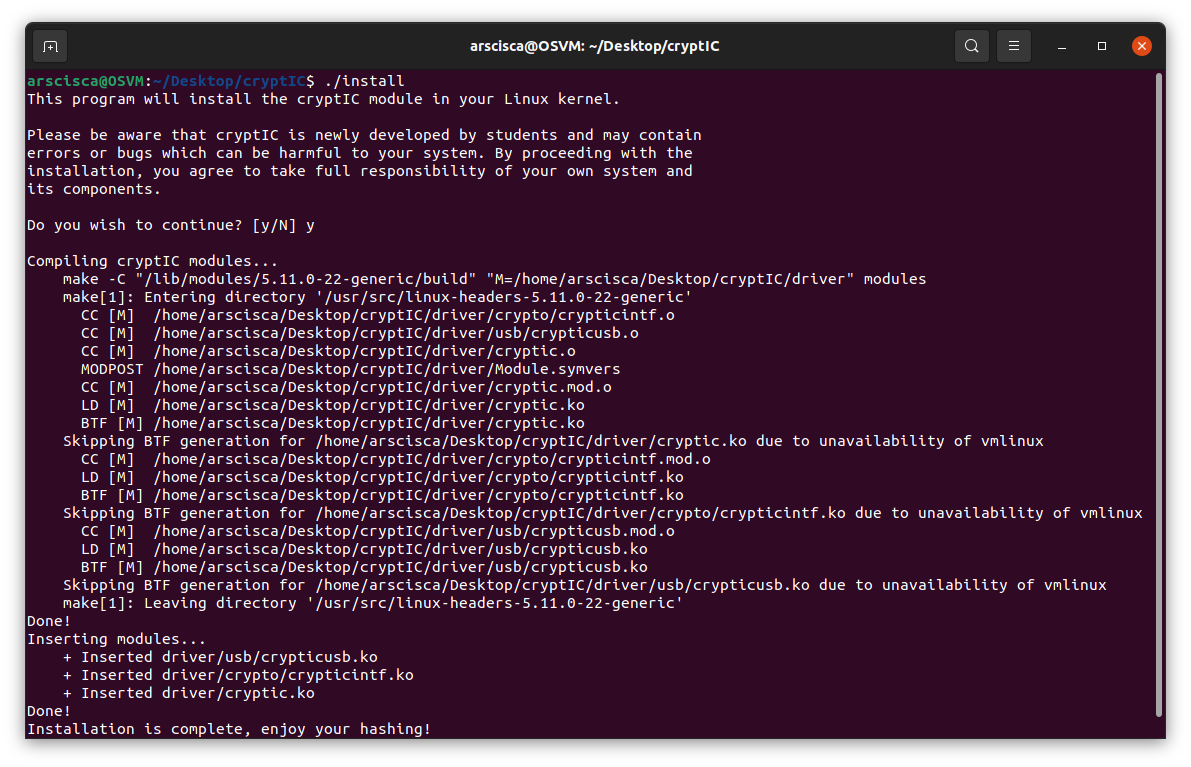
\includegraphics[width=\textwidth]{img/install.png}
		\caption{Driver installation}
\end{figure}

\begin{figure}[htb]
		\center
		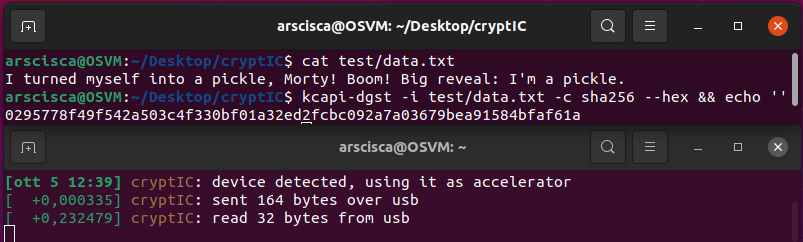
\includegraphics[width=\textwidth]{img/hash_device.png}
		\caption{Hashing example (with device connected) with \texttt{dmesg} running below showing the system messages}
    \label{img:hash_dev}
\end{figure}
\begin{figure}[htb]
		\center
		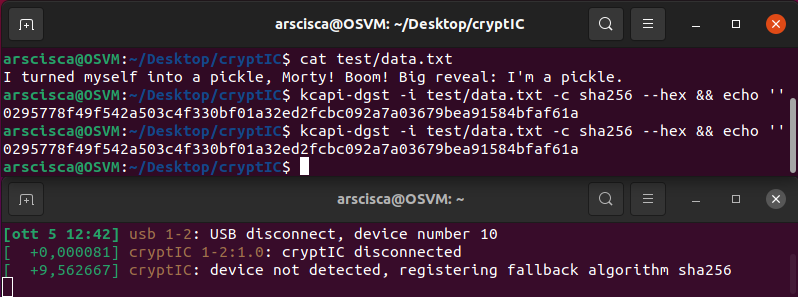
\includegraphics[width=\textwidth]{img/hash_nodev.png}
		\caption{Hashing example (with device disconnected) with \texttt{dmesg} running below showing the system messages. Notice how the second run of the command happens after the USB device had been disconnected, so the system correctly uses the fallback implementation.}
    \label{img:hash_nodev}
\end{figure}
\autoref{img:hash_dev} and \autoref{img:hash_nodev} are particularly interesting because they show the driver in action when using an external command. This shows how CryptIC is directly integrated into the Crypto Subsystem so that already existing programs can already interact with it. Moreover, this also shows how the system seamlessly handles requests even after the device is disconnected, never interrupting the user.


\begin{figure}[htb]
		\center
		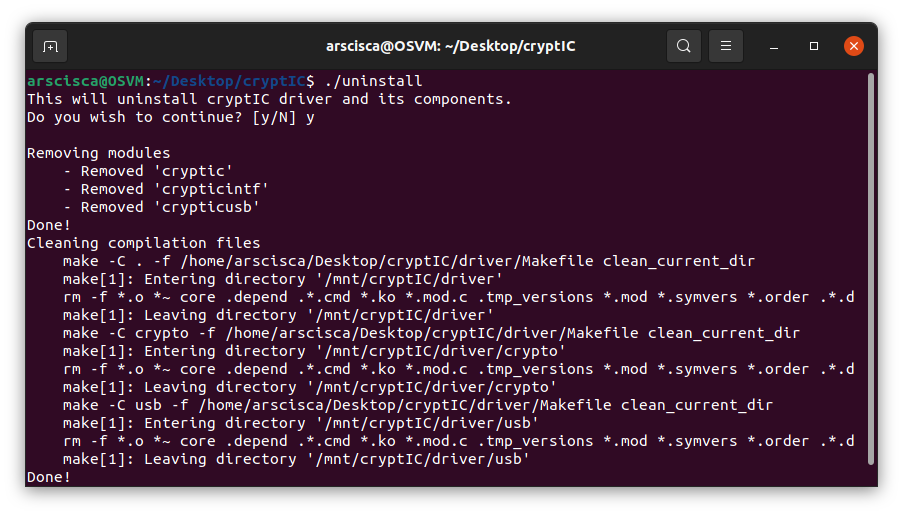
\includegraphics[width=\textwidth]{img/uninstall.png}
		\caption{Uninstalling the driver}
\end{figure}
